%
% File coling2020.tex
%
% Contact: feiliu@cs.ucf.edu & liang.huang.sh@gmail.com
%% Based on the style files for COLING-2018, which were, in turn,
%% Based on the style files for COLING-2016, which were, in turn,
%% Based on the style files for COLING-2014, which were, in turn,
%% Based on the style files for ACL-2014, which were, in turn,
%% Based on the style files for ACL-2013, which were, in turn,
%% Based on the style files for ACL-2012, which were, in turn,
%% based on the style files for ACL-2011, which were, in turn, 
%% based on the style files for ACL-2010, which were, in turn, 
%% based on the style files for ACL-IJCNLP-2009, which were, in turn,
%% based on the style files for EACL-2009 and IJCNLP-2008...

%% Based on the style files for EACL 2006 by 
%%e.agirre@ehu.es or Sergi.Balari@uab.es
%% and that of ACL 08 by Joakim Nivre and Noah Smith

\documentclass[11pt]{article}
\usepackage[utf8]{inputenc}
\usepackage{coling2020}
\usepackage{times}
\usepackage{url}
\usepackage{latexsym}
\usepackage{graphicx}
\usepackage{array}
\usepackage{hyperref}


\setlength\titlebox{5cm}
\colingfinalcopy 

\title{Advances and Problems in Reinforcement Learning \\for Natural Language Processing\\Final paper: Literature Review Article}
\author{Lisa Becker \\
        775242\\
        University of Potsdam / Am Neuen Palais 10, 14469 Potsdam, Germany \\
        {\tt lisbecke@uni-potsdam.de} \\}
\date{\today}

\begin{document}
\maketitle

\begin{abstract}
This paper dives into the current state of Reinforcement Learning for Natural Language Processing with a more specific focus on its trends, challenges and advances from related research which might improve future research of Reinforcement Learning in Natural Language Processing. A more general overview of the current state of the art of this domain can be found in Luketina et al.~\shortcite{luketina-2019-asurvey} and more specific research on the state-value in Reinforcement Learning for Natural Language processing has been provided by Madureira and Schlangen~\shortcite{madureira2020}.
\end{abstract}


\section{Introduction}
In 2016, DeepMind put Reinforcement Learning (RL) in the spotlights by developing AlphaGo~\cite{alphago}. Since then, RL has made many advances in various of its subdomains, one of them being Natural Language Processing (NLP) and is still developing.\\\\ As stated in Luketina et al.~\shortcite{luketina-2019-asurvey}, both RL and NLP influence each other. While we can gain new linguistic knowledge by getting more insight into how RL agents deal with language, NLP can be used in return to enhance RL models. Therefore, advances in RL for NLP profit both fields. Since RL in NLP started to become more popular, various subdomains and applications emerged, such as Article Summarization, Question Generation and Answering, Dialogue Generation, Dialogue Systems, Machine Translation, Text generation, recently Coreference Resolution and others, of which some will be touched in the course of this paper. This paper will first give a short introduction into the purpose of NLP in RL (Section \ref{purpose}), then it shows various Trends in NLP in RL (Section \ref{trends}) such as the evolution of Learning Algorithms, the role of Deep Learning and novel approaches regarding the Reward Function (Section \ref{learningalgo}, \ref{deeplearning} and \ref{rewardfunction}) before heading towards the Problems that NLP is facing with RL (Section \ref{problems}) and closes with a summarising Conclusion (Section \ref{conclusion}).

\section{Purpose of NLP in RL}\label{purpose}
While it is difficult to summarise the current state of using RL methods in NLP tasks (and has been done recently by Luketina et al.~\shortcite{luketina-2019-asurvey} with a specific focus on language-assisted versus language-conditional tasks), more can be said here about the purpose of RL for NLP: RL has an easier time to deal with certain difficulties of other unsupervised or supervised methods. First, it often deals better with scarce or little data. Second, it can be used to solve tasks from a different angle: Ling et al.~\shortcite{ling-etal-2017-learning} enabled RL to mimic the way a human would solve a given task, for example diagnosing an illness. Hu et al.~\shortcite{hu-etal-2018-playing} developed an RL agent that is optimised to select the correct questions to solve an answer-based game (Q20) without a knowledge base ---on which previous approaches relied--- and with more stability towards errors than previous models. \\\\
The concept of reward in RL enables us to control the training better than is possible with supervised learning. Whether the reward is given all at the end or in intervals for each action can influence training. It is also possible to focus training on several different objectives as different rewards for different things can be combined, like Mosallanezhad et al.~\shortcite{mosallanezhad-etal-2019-deep} did with one reward for anonymisation and one for usefulness. Still, the success of RL models often depends on the researcher's ability to frame the problem, particularly reward functions.\\\\
The discussion about the purpose of NLP in RL also raises the question whether language produced by machines have to sound as human as possible. While it is already possible, it poses potential danger. Jia et al.~\shortcite{ye-2018-transfer} managed to successfully and convincingly copy voices after only five seconds of input which could further be used to fake phone calls or manipulate videos. While the technique used for this approach is not RL but Transfer Learning, it shows that RL and similar approaches, like DeepFake, need to be watched closely in regard to their ethical application and new laws have to be created in order to protect from possible misuse of the new technological advances. 


\section{Trends in NLP in RL}\label{trends}
This section discusses some of the trends and novel approaches that have emerged during the past years for NLP in RL. While some tools, like REINFORCE as a Learning Algorithm, continue to be popular, there are reasons to shift to other approaches depending on the task (Section \ref{learningalgo}). \\ Deep Learning plays an important role in many NLP-related fields and RL is no exception and researchers continue to investigate its advantages for learning algorithms, state representation and reward functions (Section \ref{learningalgo}, \ref{deeplearning}, \ref{rewardfunction}). In contrast, there's a novel way of shaping rewards by turning towards supervised learning presented in this section (\ref{rewardfunction}).

\subsection{Learning Algorithms}\label{learningalgo}
\textbf{REINFORCE} is still the most commonly used learning algorithm in RL~\cite{yasui-etal-2019,zhang-2018,hu-etal-2018-playing,godin-etal-2019-learning,huang-etal-2018-neural,mao-etal-2018-end,ranzato2015sequence,wu-etal-2018-study,clark-manning-2016-deep,yogatama-2017,guu-etal-2017-language,zeng-2018}, but REINFORCE does not seem to be the optimal choice for some of them:\\\\ Clark and Manning~\shortcite{clark-manning-2016-deep} compared two models on coreferene resolution, one based on REINFORCE, the other based on a modified version of the heuristic max-margin objective introduced by Wiseman et al.~\shortcite{wiseman-etal-2015-learning} which is based on error types (correct, false new, false anaphor, wrong link) and performs hyperparameter search to choose the loss function parameters. A neural word-embedding based mention-ranking model scores pairs of mentions based on their likelihood of coreference on an English and Chinese corpus of the CoNLL 2012 Share Task ~\cite{conll-2012}. Using the MUC, B and CEAF metrics, Clark and Manning~\shortcite{clark-manning-2016-deep} found that their mention-ranking model performs well, while REINFORCE only slightly outperformed the heuristic loss, hence the authors' suggestion that REINFORCE is not an optimal choice for ranking tasks like in Grishman and Sundheim~\shortcite{grishman-sundheim-1996-message} and Cai and Strube~\shortcite{cai-strube-2010-evaluation}. They base their conclusion on REINFORCE optimising the model's performance in expectation during training, but it takes the most probable sequence of actions during testing. Generally speaking, most NLP tasks are more to be treated as sequential tasks with large, structured action spaces with discrete actions and sparse rewards, while REINFORCE ---as a method based on Monte-Carlo--- only updates after full episodes during training. In addition, REINFORCE has a heightened chance of converging to a local minimum which can lead to suboptimal results. Thus it is suggested that a shift to exploiting actor-critic methods might solve some of the aforementioned problems where the state-value function is used as a critic and thus for bootstrapping, not just as a baseline. The bias introduced by bootstrapping can be beneficial because it reduces variance and accelerates learning while REINFORCE ---as all Monte-Carlo methods--- tends to learn slowly. One reason why REINFORCE is still popular in NLP research might be that there is no need to estimate value functions and they tend to perform better on large state and action spaces than value-based methods. Still, the optimal choice for the Learning Algorithm depends on the task and can not be generalised. \\\\
A variety of other models exploit \textbf{Deep Q-Learning} instead of REINFORCE \cite{narasimhan-etal-2016-improving,mosallanezhad-etal-2019-deep,ling-etal-2017-learning} and a minority of RL models started to step away from REINFORCE by using different variations of the \textbf{policy gradient method} \cite{branavan-2009,li-etal-2018-paraphrase,li-etal-2016-deep,le-fokkens-2017-tackling} or other \textbf{actor-critic methods}, such as the ones proposed by Dethlefs and Cuayáhuitl~\shortcite{dethlefs-cuayahuitl-2011}, Grissom II et al.~\shortcite{grissom-ii-etal-2014-dont}, He et al.~\shortcite{he-etal-2016-deep-reinforcement}, Chen and Bansal~\shortcite{chen-bansal-2018-fast} and Goyal et al.~\shortcite{goyal-2019}. 

\subsection{Deep Learning in State Representation}\label{deeplearning}
Deep neural architectures are widely used to represent state in RL algorithms since they are capable of scaling to previously unsolvable problems. Applied to NLP, RL models commonly exploit RNNs in order to use the hidden vector to represent and update the environment state. An overview over the key concepts can be seen in Figure \ref{fig:states} and an extensive version of this paragraph found in Madureira and Schlangen~\shortcite{madureira2020} while a summary of it can be found below:\\

\begin{figure}[h!]
\centering
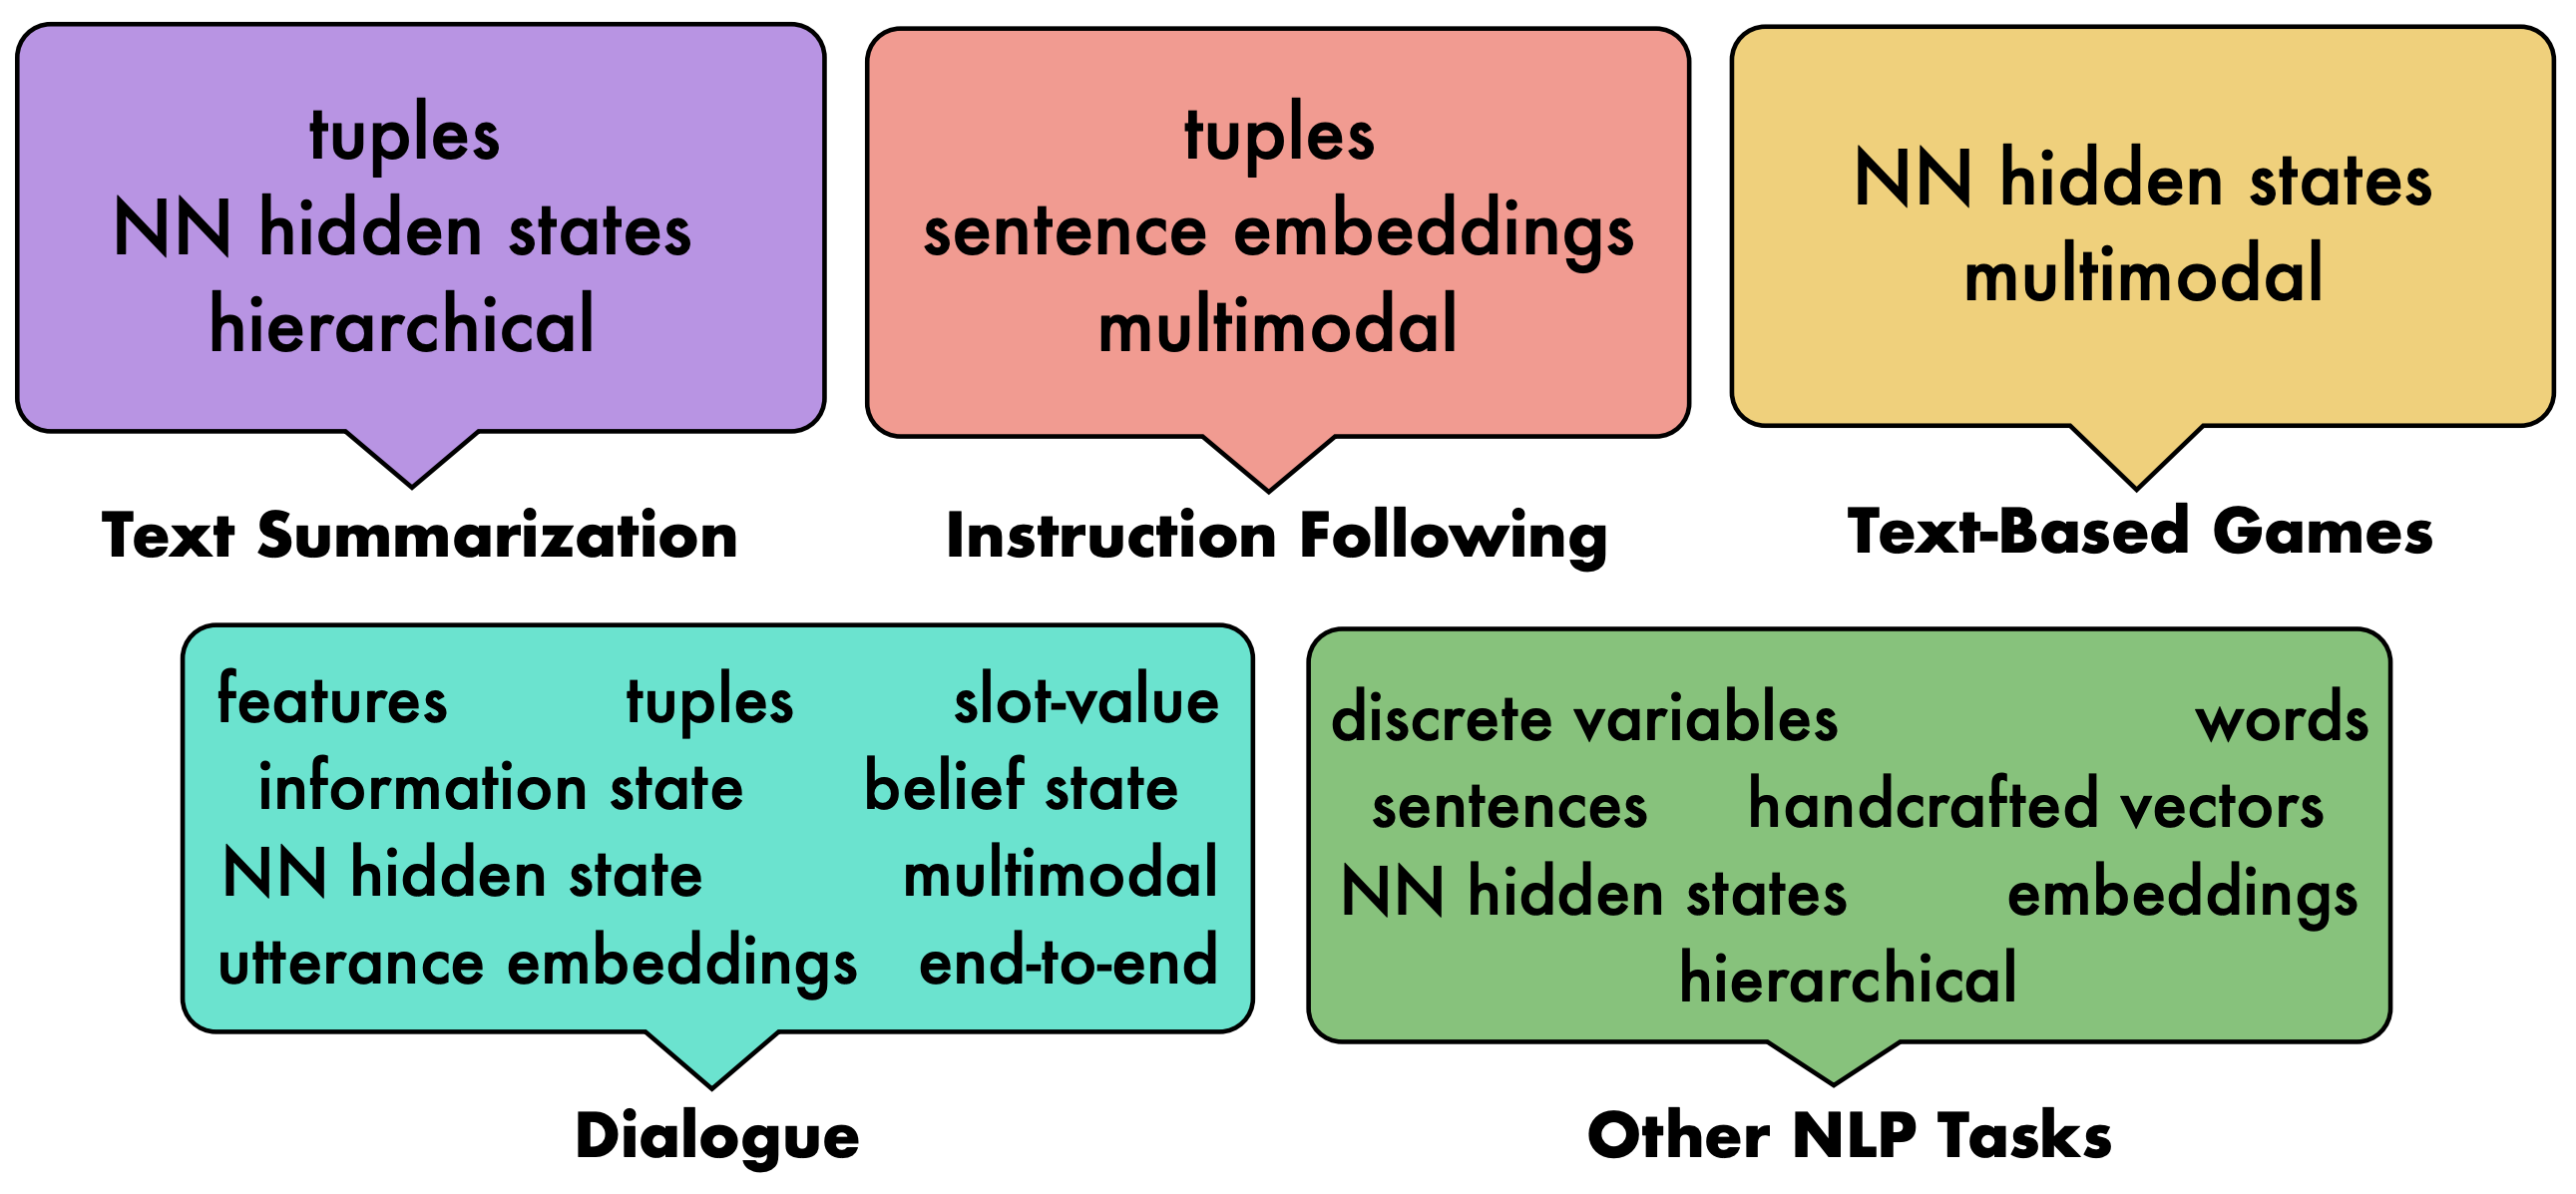
\includegraphics[scale=.3]{img/states.png}
\caption{Overview over the key concepts of state representation per subdomain. Not all concepts are represented by example in this paper. Figure from Madureira and Schlangen~\shortcite{madureira2020} where the full analysis of state representations can be found.}
\label{fig:states}
\end{figure}
\begin{itemize}


\item \textbf{Text Summarisation} is achieved by Natural Language Generation models generating a summary of a text with new words or a model that chooses the most relevant sentences. Deep Learning helped RL becoming a more prevalent method for text summarisation: the state representation is encoded as the hidden state of the RNN which composes the summary \cite{ling-etal-2017-learning}. \\ A hierarchical approach can be realised by global information being captured by a CNN at sentence level and an LSTM or BiLSTM at document level \cite{chen-bansal-2018-fast}.
\item \textbf{Instruction Following} ---the process of choosing an action based in textual input--- was realised by Branavan et al.~\shortcite{branavan-2009} by mapping world features to words and linguistic features to documents where the tuple or word and document represents the state.
\item \textbf{Text-Based Games} were built by He et al.~\shortcite{he-etal-2016-deep-reinforcement} by using neural networks in order to build continuous vectors: the semantic of the game state was represented by an LSTM over textual data with a mean pooling layer.\\ LSTMs, or bag of words, were used by Narasimhan et al.~\shortcite{narasimhan-2018} to concatenate an object with its textual specification embedding to factorise state representation.
\item \textbf{Dialogue systems} were realised with LSTMs by Li et al.~\shortcite{li-etal-2016-deep} (among others) by using the two previous dialogue turns and transforming them into a continuous vector representation with the help of an LSTM encoder in order to build representations from raw text. 
\item \textbf{Other NLP Tasks} consisted of various different applications: a number of studies used vectors to represent the state, for example Narasimhan et al.~\shortcite{narasimhan-etal-2016-improving}, who used td-idf and one-hot encoding of matches for \textbf{information extraction}, Dethlefs and Cuayáhuitl~\shortcite{dethlefs-cuayahuitl-2011}, who used situational and linguistic information for \textbf{natural language generation}, Godin et al.
~\shortcite{godin-etal-2019-learning} worked with entities and relations in the domain of \textbf{question answering} and Hu et al.~\shortcite{hu-etal-2018-playing} build a model for \textbf{question selection} by using the probability distribution over a set of objects. Lê and Fokkens~\shortcite{le-fokkens-2017-tackling} described the state of a parse structure with a parser configuration as a set of discrete variables for \textbf{semantic parsing}.
Clark and Manning~\shortcite{clark-manning-2016-deep} used word embeddings and features to solve \textbf{coreference resolution}. Grissom II et al.~\shortcite{grissom-ii-etal-2014-dont} used predicted words for simultaneous \textbf{machine translation}, Mao et al.~\shortcite{mao-etal-2018-end} used a vocabulary set and a taxonomy for \textbf{taxonomy induction}.\\
The state representation has been implemented with the help of RNNs by using the RNN as the agent and the hidden state as the environment. This was done by the following studies: Yasui et al.~\shortcite{yasui-etal-2019} and Ranzato et al.~\shortcite{ranzato2015sequence} used LSTMs as the environment state for \textbf{natural language generation} and \textbf{image captioning}. \\ Yogatama et al.~\shortcite{yogatama-2017} used a combination of hidden states and another neural network for \textbf{sentence representation} while Wu et al.~\shortcite{wu-etal-2018-study} used a Transformer's hidden states for \textbf{machine translation}. Guu et al.~\shortcite{guu-etal-2017-language} and Mosallanezhad et al.~\shortcite{mosallanezhad-etal-2019-deep} made use of the output layer's encoding for semantic parsing and in combination with location-based attention in text anonymisation.
\end{itemize}

As seen by the variety of models using different deep learning structures, RNNs seem to become more popular for encoding and decoding text, but there is also a trend towards the use multimodal or hierarchical representations and or end-to-end models.

\subsection{Reward Function}\label{rewardfunction}
While common evaluation metrics (also see Section \ref{evaluation}) are often used as feedback in the reward function to improve the model's performance during training \cite{ranzato2015sequence,wu-etal-2018-study,grissom-ii-etal-2014-dont,chen-bansal-2018-fast} or self-shaped rewards, there is one novel approach which deviates strongly from previous methods and which will be discussed in detail:\\\\
Schmidhuber~\shortcite{schmidhuber2019reinforcement} suggested a reward function called \textbf{Upside Down RL (UDRL)}. In comparison to traditional RL which predicts rewards, UDRL turns the algorithm into a form of supervised learning by using environmental rewards as task-defining inputs rather than the learning target (see Figure \ref{fig:udrl}). It interprets input observations as commands and maps them to actions. First experiments with UDRL show that this novel approach can outperform traditional baseline algorithms on certain RL tasks, such as the LunarLander-v2 and the TakeCover-v0 games (see Figure \ref{fig:udrl_games}) \cite{srivastava2019training,openaigym,vizdoom}. Their model trains an agent model-free, thus without value-based or policy-based algorithms but instead uses supervised learning to train the agent on past experience, including function approximation, bootstrapping and off-policy training.\\\\
Less solely related to the reward function is Schmidhuber's~\shortcite{schmidhuber2019reinforcement} other approach for teaching a robot to imitate humans:\\ Based on the \textbf{Imitate-Imitator concept}, parents imitate the babbling of their babies and use child-directed speech. Robots learned through supervised learning how humans imitate the robots' current behaviour by mapping a video which functions as input commands. Afterwards, they were supposed to generalise and imitate videos of humans executing new behaviour. This model could be applied to any sequential or multi-modal sensory data (including spoken commands or gestures) from which the desired behaviour can be described to an RNN, thus its relevancy for NLP. 

\begin{figure}[h!]
\centering
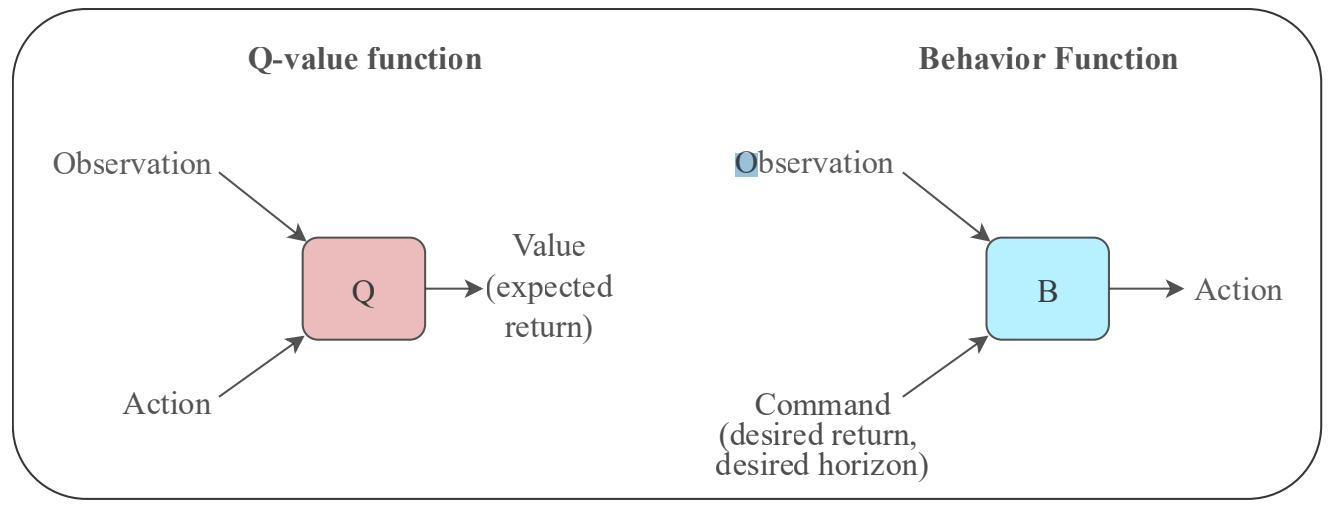
\includegraphics[scale=.42]{img/udrl_graphic.PNG}
\caption{Key distinction between traditional RL and UDRL: the roles of actions and returns are switched while UDRL can have additional command inputs. Figure from Srivastava et al.~\shortcite{srivastava2019training}.}
\label{fig:udrl}
\end{figure}

\begin{figure}[h!]
\centering
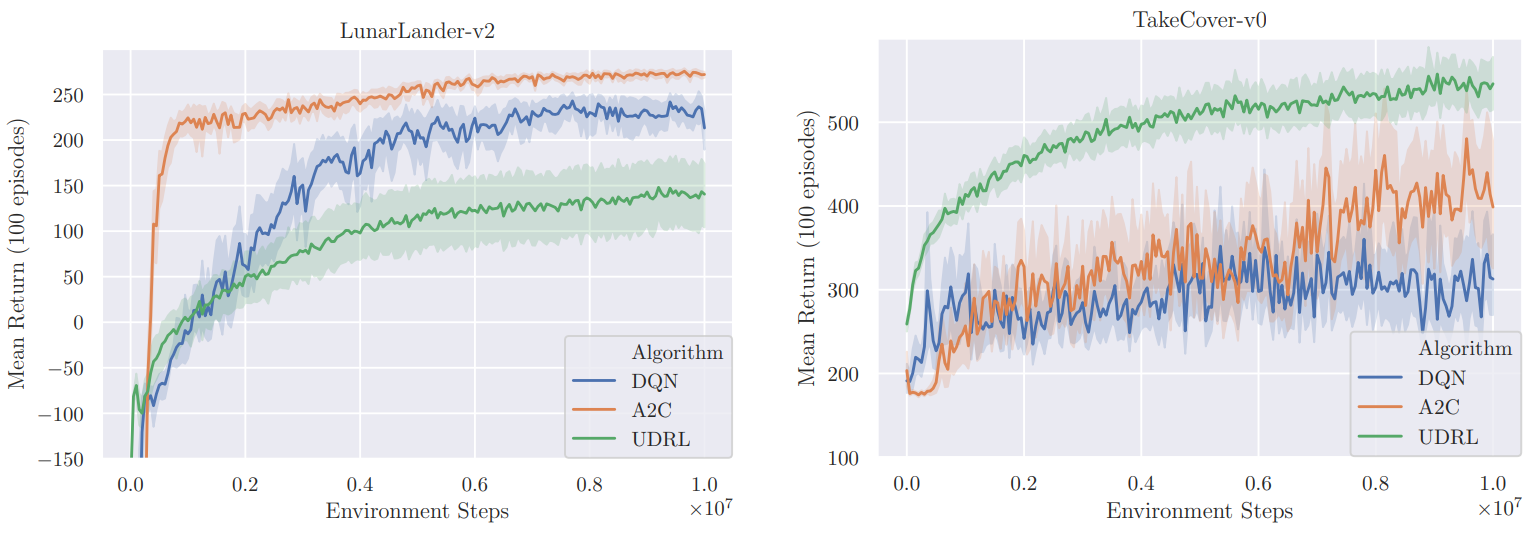
\includegraphics[scale=.39]{img/udrl_test_image.PNG}
\caption{Srivastava et al.~\shortcite{srivastava2019training} tested a pilot implementation of UDRL against the more traditional Deep Q-Learning (DQL) and an Advantage Actor-Critic (A2C, from \cite{mnih-2015}) on two test environments well known for RL: LunarLander-v2 and TakeCover-v0, available in the Open AI Gym and VizDoom~\cite{openaigym,vizdoom}. It can be seen that UDRL outperforms other approaches in the TakeCover-v0 task very early and tends to be more stable in general. Figures from Srivastava et al.~\shortcite{srivastava2019training}.}
\label{fig:udrl_games}
\end{figure}
\newpage

\section{Problems for NLP in RL}\label{problems}
Research is facing a few problems regarding the application of RL in NLP which spans across a large range of studies. First, there is a short introduction into the relevancy of the different parts of an RL model with attention to the state (Section \ref{state}), then the importance of the data and the language in which research is conducted is discussed in respect to research in general (Section \ref{data}). Afterwards, knowledge representation and specifically grounding in RL are investigated (Section \ref{knowledgerepresentation}) and lastly, different ways to evaluate RL models for NLP are discussed (Section \ref{evaluation}).

\subsection{State Representation}\label{state}
While most research focuses on improving the reward function in order to maximise the agent's expected long-term reward and describes their implementation of such in detail in the respective paper, Madureira and Schlangen~\shortcite{madureira2020} discussed the importance of \textbf{state} and its representation in RL for NLP. While the formalisation of the state and its properties depends on the value and reward function, vice versa and thus form an arguably equally important part of an RL model, there is still less attention directed towards the state. This shows for example in the fact that many researchers neglect describing their state signal and the reasoning of their choice for the state representation, which alone makes understanding and replicating their models more difficult. With the rise of neural network models in RL for NLP, states could be more easily represented by a vector and thus more easily fed into the value or policy function. Madureira and Schlangen~\shortcite{madureira2020} appealed for more linguistically interpretable and grounded state representations next to encouraging researchers to pay more attention to the choice of their state function, its explanation and respective evaluation in the paper. While this seems to be especially problematic for the state representation, the lack of detailed description can span across all parts of RL research.

\subsection{Data and Language}\label{data}
\textbf{Anglocentrism} dominates most research fields, with NLP and more specifically RL being no exception. This is due the general relevancy of the English language and hence it being the main language in which research is written and communicated. While this is not a problem per se, it compels many researchers to also use English as their main language for conducting their experiments due to available data and funding for research regarding the English language. This homogeneity is a common property of any, but particularly of young research fields which still needs to be overcome by broadening up and paying more attention to other languages. This is not only important in terms of ethical diversity but also a necessary step to achieve overall application of RL across languages. The focus on English data limits the possible new insights that RL and other research fields could provide us.\\\\
\textbf{Data} is not only limited in language but also in size and diversity. Since models which exploit deep learning (like some RL models) tend to improve with larger corpora, it becomes exponentially difficult to provide data sets of sufficient quality by the increase of size. Consequently, many experiments are performed on the same old data sets which are mostly available in English. The few studies that concern languages other than English are usually regarding machine translation and still contain English, for example between English and German~\cite{yasui-etal-2019}. \\\\
To tackle the problem of data set availability, some RL agents became more specialised on performing well on \textbf{smaller data sets} by using a document name and specific keywords to search the internet for additional documents which contain similar information ~\cite{narasimhan-etal-2016-improving}. The entities get categorised by ensuring that the entity class predictions are compatible and consistent between different sources. The RL agent evaluates how well the search process is going and determines whether it should continue or stop.\\\\
While there is a wide range for data augmentation on visual data, there are not many reliable \textbf{augmentation models for linguistic data}. There are a few exceptions, for example Yoon et al.~\shortcite{yoon-2018-pategan} who propose an domain-independent approach for synthesising data with GANs (without being specifically RL related). Methods like these might not only help expanding the range of data sets but also make it easier for researchers to construct their own ones to fit the specific application of their RL model.\\\\
Some newer and more innovative data sets have not been created specifically for training RL models but can be exploited for training them, such as the SCONE (Sequential CONtext-dependent Execution) introduced by Long et al.~\shortcite{long-2016} and have been applied to RL by Guu et al.~\shortcite{guu-etal-2017-language}. The SCONE data set spans three different domains which do not include semantic annotations but only world states. Therefore it makes training ambiguous while the RL agent develops a strategy to navigate the "Alchemy", "Tangrams" and "Scene" problems.\\\\
Lastly, projects like Amazon Mechanical Turk\footnote{\hyperlink{https://www.mturk.com/}{Amazon Mechanical Turk}, "is a crowdsourcing marketplace that makes it easier for individuals and businesses to outsource their processes and jobs to a distributed workforce who can perform these tasks virtually", last accessed 2020-09-13.} and DefinedCrowd\footnote{\hyperlink{https://www.definedcrowd.com/}{DefinedCrowd} is a company which provides purchasable data for scientists which is acquired and validated by a global community, similar like Amazon Mechanical Turk, last accessed: 2020-09-07} help with providing larger data sets generated and annotated by humans for different purposes since it allows researchers to have access to a large and diverse population ~\cite{AMTurk-2012}. 

\subsection{Knowledge Representation}\label{knowledgerepresentation}
It is not only crucial for science in which language data is available but also how language is generally implemented in the the RL model. Knowledge representation describes how real-life ---or human--- knowledge is encoded ---or represented--- in a way that the model understands it and can use it to solve complex problems. An example of knowledge representation is the encoding of pictures or language.\\\\
\textbf{Grounding} ---connecting or relating language to the real world--- is dependent on the representation of knowledge and will become one of the key features in future RL research according to Narasimhan et al.~\shortcite{narasimhan-2018}. While mainly prevalent in the intersection between language and vision, both aspects need to be encoded in a way that an RL agent can utilise it, the balance has to be found between modifying language and leaving it in its natural state such that the bridge between RL agents and the real world can be crossed. The importance of grounding also depends on whether the RL agent has to solve a language-conditional or a language-assisted task, as Luketina et al.~\shortcite{luketina-2019-asurvey} stated: grounding is more crucial to language-conditional cases in order to exhibit underlying understanding. For language-assisted tasks, RL model can use natural language to improve their baseline or reward function. Advancing methods for grounding could make a significant different for real life applications or RL in NLP as well as give new linguistic insights. In order to improve grounding, Luketina et al.
~\shortcite{luketina-2019-asurvey} suggested that there should be more focus on learning from natural, diverse corpora instead of following instructions and small and synthetic corpora. While it is more difficult, the application range is much broader. In order to achieve that, they advised to pay more attention to pre-training language models, general advances in representation learning and the development of tools for more diverse RL environments to better reflect reality. Lastly, appropriate grounding is crucial for RL agents that need to interact with the real world. To pass the Turing test, an agent might only have to produce a coherent conversation. But if RL agents, for example in the form of nursing assistants, need to keep people company, educate them or keep them save, they need to be aware of the surroundings and have to be able to set into a context in order to react accordingly to a situation or conversation. 

\subsection{Evaluation measures}\label{evaluation}
The choice of evaluation measures is especially problematic in RL agents which generate language. On one hand, automating evaluation is complex and unreliable but on the other hand, human evaluation is very inefficient in time and resources. Some attempts have been made to combine both approaches, although not in the domain of RL but in a neural paraphrasing model~\cite{goyal-durrett-2020-neural} by simply applying both a quantitative and a human evaluation on the data and combining the scores. \\\\
Although already introduced in 2002 or shortly after, many recent studies still evaluate with the \textbf{Bilingual Evaluation Understudy (BLEU)}, \textbf{Recall-Oriented Understudy for Gisting Evaluation (ROUGE)} or \textbf{Metric for Evaluation of Translation with Explicit ORdering (METEOR)} ~\cite{lin-2004-rouge,banerjee-lavie-2005-meteor} despite new ways of evaluating being introduced, for example by the yearly metrics challenge by the WMT conference\footnote{\hyperlink{http://www.sigmt.org/}{WMT (Workshop on statistical Machine Translation) is a yearly held metrics challenge by the Special Interest Group for Machine Translation}, last accessed 2020-09-13.}. While there is evidence for BLEU's validity in predicting human judgements~\cite{reiter-2018-astructured}, Reiter\footnote{Ehud Reiter discusses this on his personal blog:\\ --- \hyperlink{https://ehudreiter.com/2020/03/02/why-use-18-year-old-bleu/}{"Why do we still use 18-year old bleu?"}, last accessed 2020-09-13. \\ --- \hyperlink{https://ehudreiter.com/2020/07/28/small-differences-in-bleu-are-meaningless/}{"Small differences in bleu are meaningless"}, last accessed 2020-09-13.} and others also found that BLEU and similar evaluation methods are outdated and should not be used for evaluating Natural Language Generation ~\cite{reiter-2018-astructured,mathur-etal-2020-tangled}. This is because BLEU is checking for matching ngrams in generated and texts written or annotated by humans. With the evolution of Machine Translating, variation of text becomes more important, which is not what BLEU is optimised for. A well varied text would decrease ratings from BLEU and similar metrics which reward systems which consistently use a specific wording and syntax. Hence, human preference is the opposite of BLEU's preference. BLEU also tends to perform worse on models that use languages like German in Machine Translation or other NLP applications for a similar reason: the word order in German is relatively free compared to English and Romance languages which impacts the reliability of BLEU\footnote{Ehud Reiter discusses this on his personal blog: \\ --- \hyperlink{https://ehudreiter.com/2018/06/20/bleu-in-different-languages/}{"Bleu   in   different   languages"}, last accessed 2020-09-13.}.\\\\
There is a novel attempt to improve BLEU by combining it with Bidirectional Encoder Representations from Transformers (BERT) and make it more robust for human judgement, called \textbf{Bilingual Evaluation Understudy with Representations from Transformers (BLEURT)}~\cite{papineni-etal-2002-bleu,sellam2020bleurt}. BLEURT generalises the model in pre-training with millions of synthetic examples. The authors claim that their model is robust and reaches an unprecedented level of quality which is closer to human evaluation than previous models. Another new approach exploiting BERT has been tested to \textbf{automatise evaluation}: Yasui et al.~\shortcite{yasui-etal-2019} trained a BERT-model to recognise semantically similar sentences of a translation model. Here we see that machine translated sentences can achieve human performances, but human translation is still superior when it spans more than one sentence: humans prefer variety in syntax and choice of words for longer text which is not yet given by this model. \\\\
Motivated by the instability of automatic evaluation methods for NLG (although used in 80\% of empirical papers presented at the ACL track on Natural Language Generating (NLG) of INLG\footnote{\hypertarget{https://www.inlg2020.org/}}{International Conference for Natural Language Generation (INLG), last accessed 2020-09-14.} in 2018 versus 3\% using extrinsic human evaluation) van der Lee et al.~\shortcite{van-der-lee-etal-2019-best} evaluated different evaluation methods against each other, since there is no consensus yet of how (NLG) systems should be evaluated by humans. They argue against automated metrics with their uninterpretability and that they do not correlate with human evaluation. In their paper, they give an overview over existing human evaluation models and summarise a set of best practices for human evaluation in NLG (see Table \ref{table:1}):\\

\begin{table}[h!]
\begin{center}
\begin{tabular}{m{7em}m{12cm}}
 \textbf{Topic} & \textbf{Best practice}  \\ \hline
 General & Always conduct a human evaluation (if possible).  \\  \hline
 Criteria & Use separate criteria rather than an overall quality assessment.
Properly define the criteria that are used in the evaluation. \\\hline
Sampling & Preferably use a (large-scale) reader-focused design rather than a (small-scale) expert-focused design.
Always recruit sufficiently many participants. Report (and motivate) the sample size and the demographics. \\\hline
Annotation &  For a qualitative analysis, recruit multiple annotators (at least 2, more is better)
Report the Inter-Annotator Agreement score with confidence intervals, plus a percentage agreement. \\\hline
Measurement & For a quantitative study, use multiple item 7-point (preferably) Likert scales, or (continuous) ranking. \\\hline
Design &  Reduce order- and learning effects by counterbalancing/random ordering, and properly report this. \\\hline
Statistics & If the evaluation study is exploratory, only report exploratory data analysis.
If the study is confirmatory, consider preregistering and conduct appropriate statistical analyses.
\end{tabular}
\caption{List of best practices for human evaluation of automatically generated text from van der Lee et al.~\shortcite{van-der-lee-etal-2019-best}.}
\label{table:1}
\end{center}
\end{table}

In paraphrase generation, Li et al.~\shortcite{li-etal-2018-paraphrase} proposed training their own evaluators (together with a generator) by two different models, \textbf{Reinforced by Matching-Supervised Learning (RbM-SL)} and \textbf{Reinforced by Matching-Inverse Reinforcement Learning (RbM-ISL)}. The method reminds of General Adversarial Networks (GANs) with the difference being that "GANs employ the discriminator to distinguish generated examples from real ones while RbM-IRL employs the evaluator as a reward function in RL. The generator in GAN is trained to maximise the loss of the discriminator in an adversarial way, while the generator in RbM-IRL is trained to maximize the expected cumulative reward from the evaluator". Each models perform better at a different task: RbM-SL performs better on a Quora data set because it can make use of the additional labelled data to train the evaluator. RbM-IRL performs better on the Twitter data because its evaluator deals better with a smaller data than its counterpart, thus RbM-SL scores better on the relevancy measure and RbM-IRL better on fluency.

\section{Conclusion}\label{conclusion}
RL would in the future not only profit from innovative methods but also from researchers being more careful in their choice of models and their description in the paper such that it is better accessible and easier to reproduce by peers. Similarly, more attention towards grounding and knowledge representation could be a crucial step towards more utile RL agents and their application to more general tasks.\\\\
More data sets of high quality and large size, a diverse range of languages which are free of charge might improve future studies and make research more accessible. Projects like Amazon Mechanical Turk and DefinedCrowd opened a new door for research but are still hidden behind a paywall which is a disadvantage for research because not everybody who would want to work with the data is able to. Additionally, there has to be a shift from anglocentrism to investigate other languages with RL in order to gain new understandings of the specific languages and language in general which will in return benefit the models and direct applications of RL in a bigger context.\\\\
New approaches to shape the reward function, like the UDRL from Schmidhuber~\shortcite{schmidhuber2019reinforcement} might be able to improve the research in certain subdomains of NLP but more studies have to be conducted to evaluate the potential of UDRL.\\\\
While most studies still make use of older evaluation metrics like BLEU, ROUGE or METEOR, there is a shift happening: older metrics get a make over and or get combined with new approaches, like Sellam et al.'s ~\shortcite{sellam2020bleurt} BLEURT, or combining the evaluator with the reward function ~\cite{li-etal-2018-paraphrase} for paraphrase generation or the yearly metrics challenge from the WMT by the SIG MT. RbM-SL and RbM-IRL need to be applied to more experiments to evaluate their potential.\\
For human evaluation, research might benefit from a standardised procedure like the one proposed by van der Lee et al.~\shortcite{van-der-lee-etal-2019-best} in Table \ref{table:1}.\\\\
As Luketina et al.~\shortcite{luketina-2019-asurvey} stated, "approaches combining language and RL will find applications as wide-ranging as autonomous vehicles, virtual assistants and household robots". While RL in NLP has made some advances, it is still far from being successfully exploited in Life Sciences. More careful research, especially in regard to the limitations and ethical implications, has to be conducted in order to model agents who can reliably applied to everyday life. Subsequently, the appropriate environment has to be formed in the sense of new regulations and laws in parallel to the rise of technological applications. 

\newpage
\bibliographystyle{coling}
\bibliography{coling2020}

\end{document}
